\section{Grad-CAM}
Grad-CAM\cite{selvaraju2017grad} (Gradient-weighted Class Activation Mapping) is a white box method, it requires insight into the convolutional neural network architecture and is therefore only applicable on CNNs. The method generates a heat map similar to RISE. Figure \ref{grad_cam_dog} and Figure \ref{grad_cam_cat} show an example output of Grad-CAM.

\begin{figure}[H]
    \centering
    \begin{subfigure}{.5\textwidth}
        \centering
        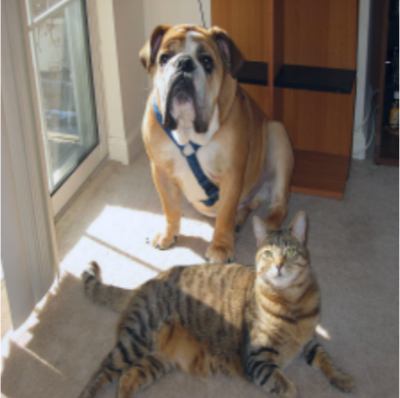
\includegraphics[width=0.7\linewidth]{chapters/02_methods/images/grad-cam-original.png}
        \caption{Original image}
    \end{subfigure}\hfill%
    \begin{subfigure}{.5\textwidth}
        \centering
        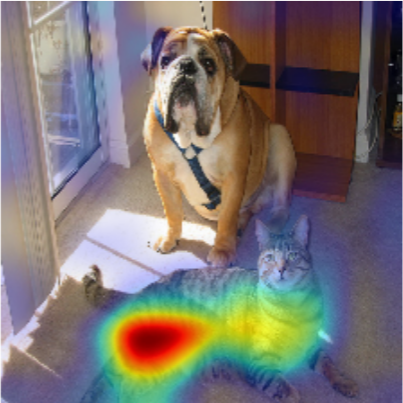
\includegraphics[width=0.7\linewidth]{chapters/02_methods/images/grad-cam-cat.png}
        \caption{Grad-CAM explanation for class cat}
    \end{subfigure}
    \caption{Grad-CAM applied on an image with multiple valid classes. Explanation for class cat.}
    \label{grad_cam_cat}
\end{figure}

\begin{figure}[H]
    \centering
    \begin{subfigure}{.5\textwidth}
        \centering
        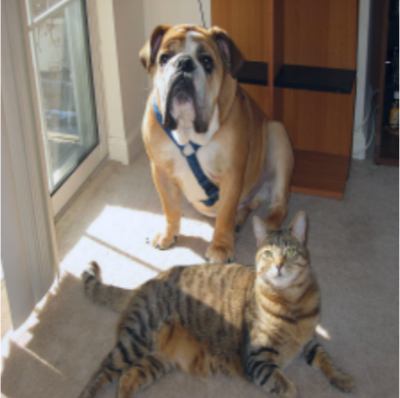
\includegraphics[width=0.7\linewidth]{chapters/02_methods/images/grad-cam-original.png}
        \caption{Original image}
    \end{subfigure}\hfill%
    \begin{subfigure}{.5\textwidth}
        \centering
        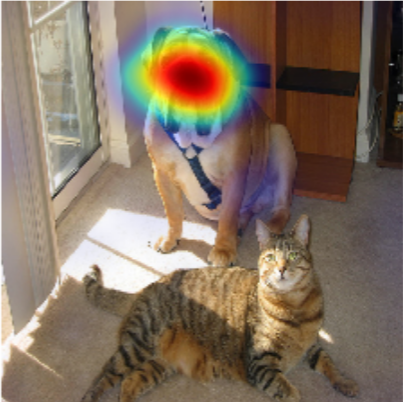
\includegraphics[width=0.7\linewidth]{chapters/02_methods/images/grad-cam-dog.png}
        \caption{Grad-CAM explanation for class dog}
    \end{subfigure}
    \caption{Grad-CAM applied on an image with multiple valid classes. Explanation for class dog.}
    \label{grad_cam_dog}
\end{figure}

The main parameter for this method is which layer of the convolutional neural network that should be analyzed. Figure \ref{grad_cam_explanation} shows a schematic of the inner working of Grad-CAM: The feature map of the specified layer is extracted. Every channel of the feature map is weighted, based on how much it influences the final output value of the network for a specific class.



There are many existing implementations for this method, some of them using the PyTorch library.

TODO: how does it work?


* works on a specific layer of the neural network
* get feature map for every channel of this layer
* sum up feature map
* based on output class, so activation has to flow backwards

So, to explain in simple terms, we simply take the final convolutional feature map and then we weigh every channel in that feature with the gradient of the class with respect to the channel. It’s just nothing but how intensely the input image activates different channels by how important each channel is with regard to the class. The best part is it doesn’t require any re-training or change in the existing architecture.


\begin{figure}[H]
\centering
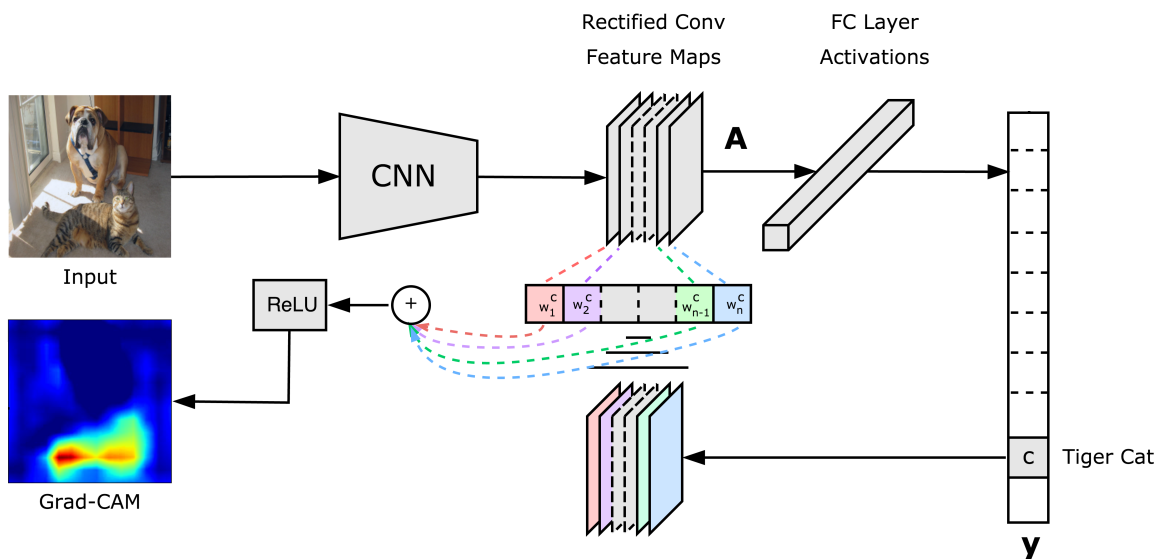
\includegraphics[width=12cm]{chapters/02_methods/images/grad-cam.png}
\caption{Grad-CAM in action: The feature map of a specific network layer is extracted, each channel weighted by the activation of the expected class, then summed up and converted into a heat map}
\label{grad_cam_explanation}
\end{figure}

